\documentclass{beamer}
\usetheme{Boadilla}
\usecolortheme{spruce}

\usepackage{default}

\title{VREP pathfinding using A* algorithm}
\author[Szilagyi Ervin]{Szil\'{a}gyi Ervin}
\institute{Sapientia EMTE}

\begin{document}
	
	\begin{frame}
		\titlepage
	\end{frame}
	
	\begin{frame}
		\frametitle{Introduction}
		\begin{itemize}
			\item This project's goal is to develop a controller for a mobile car-like robot. The aim is to drive the robot from point A to point B following a given path.
			\item
			The project is developed in C++14 using the following additional libraries:
			\begin{itemize}
				\item Boost version 1.58.0
				\item OpenCV 2.4
				\item VREP Remote API 
			\end{itemize}
		\end{itemize}
	\end{frame}
	
	\begin{frame}
		\frametitle{A* algorithm}
		\begin{equation}
			f(n) = g(n) + h(n)
		\end{equation}
		Where $n$ is the final node, $g(n)$ is the cost of the path from start point to $n$ and $h(n)$ is a heuristic function.
		$g(n)$ can be calculated using euclidean distance from $n$ to the finishing point:
		\begin{equation}
		g(n) = \sqrt{(x_1 - x_2)^2 + (y_1 - y_2)^2}
		\end{equation}
		$h(n)$ is a heuristic function which represents the numbers of steps done from the starting point to $n$:
		\begin{equation}
		h(n) = step(0..n)
		\end{equation}
	\end{frame}
	
	\begin{frame}
		\frametitle{Main scene}
		\begin{figure}
			\centering
			\begin{minipage}[b]{0.4\textwidth}
			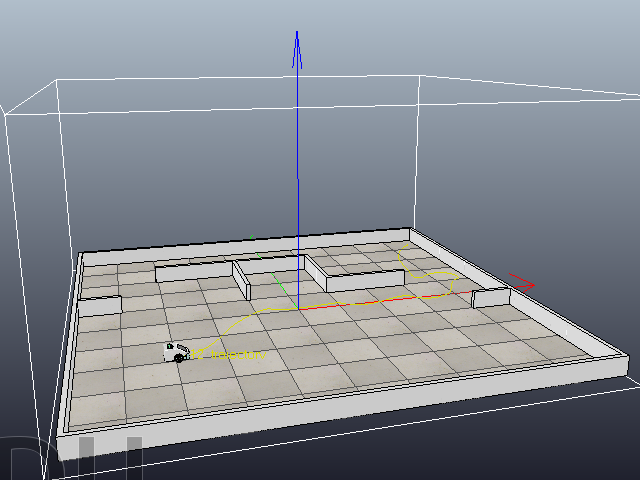
\includegraphics[scale=0.25]{scene}
			\centering
			\caption{Main scene with vision sensor}
			\end{minipage}
			\hfill
			\begin{minipage}[b]{0.4\textwidth}
			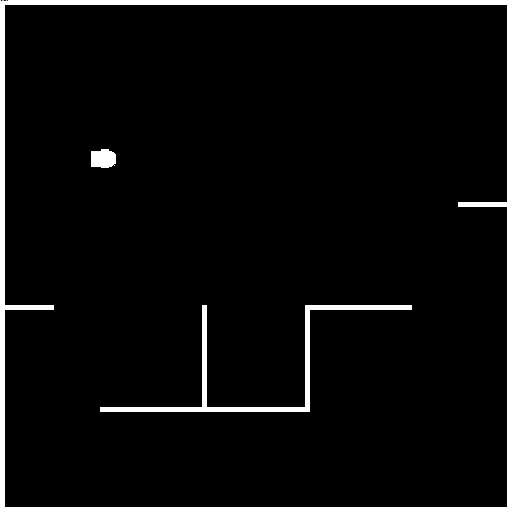
\includegraphics[scale=0.35]{original}
			\centering
			\caption{Vision sensor image}
			\end{minipage}
		\end{figure}
	\end{frame}
	
	\begin{frame}
		\frametitle{Image processing and finding a path}
	\begin{figure}
		\centering
		\begin{minipage}[b]{0.4\textwidth}
			
\includegraphics[scale=0.35]{dilated}
			\centering
			\caption{After processing (robot's figure deleted, image dilated)}
		\end{minipage}
		\hfill
		\begin{minipage}[b]{0.4\textwidth}
			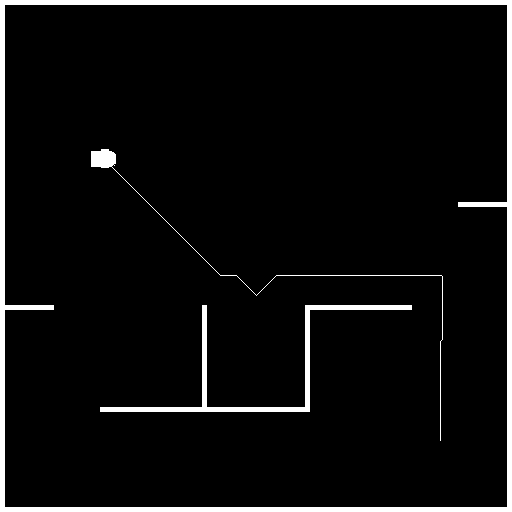
\includegraphics[scale=0.35]{with_path}
			\centering
			\caption{With final path}
		\end{minipage}
	\end{figure}
	\end{frame}
	
	\begin{frame}
		\frametitle{Robot controller}
		\begin{figure}
			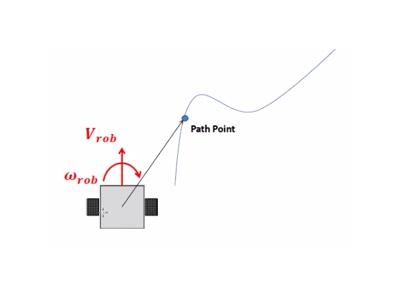
\includegraphics[scale=0.5]{controller}
			\caption{Robot controller}
		\end{figure}
	\end{frame}
	
	\begin{frame}
		\frametitle{Implementation of the controller}
		The velocity of the right and left wheels is:
		\begin{equation}
		speedRight = speed + d * rotationSpeed * orientation;
		\end{equation}
		\begin{equation}
		speedLeft = speed - d * rotationSpeed * orientation;
		\end{equation}
		where $d$ is the distance between the wheels. \\
		The wheel rotation velocities are:
		\begin{equation}
		\omega_r = speedRight / r;
		\end{equation}
		\begin{equation}
		\omega_l = speedLeft / r;
		\end{equation}
		where $r$ is the radius of the wheels.
	\end{frame}
	
	\begin{frame}
		\frametitle{References}
		\begin{itemize}
			\item Nikolai K. - 03: Path Planning with a Differential Drive Robot | V-Rep Tutorial (https://www.youtube.com/watch?v=OfpB87pRoUk)
			\item Claudiu Popirlan, Mihai Dupac - An Optimal Path Algorithm for Autonomous Searching
			Robots
		\end{itemize}
		\vspace{1cm}
		\centering
		Source code and documentation of this project can be found here: https://github.com/Ernyoke/VREP\_Pathfinding.git
	\end{frame}

\end{document}
